\chapter{Filtering methods}
\label{sec:filter}

In this chapter, I present various filtering methods for approximate string matching.
I consider two classes of filtering methods: those based on \emph{seeds} and those based on \emph{$q$-grams}.
Filters of the former class partition the pattern into \emph{non-overlapping} factors called seeds, while filters of the latter class consider all \emph{overlapping} substrings of the pattern having length $q$, the so-called $q$-grams.
Both classes include various combinatorial filtering methods of increasing specificity and complexity, always providing filtration schemes with guarantees on filtration sensitivity.

I consider the following seed filtering methods:
%\begin{inparaenum}[(i)]
\emph{exact seeds} \citep{Baeza1992},
\emph{approximate seeds} \citep{Myers1994,Navarro2000},
\emph{suffix filters} \citep{Kaerkkaeinen2007}.
%\end{inparaenum}
Exact seeds partition the pattern in $k+1$ non-overlapping seeds, to be searched exactly.
Approximate seeds increase specificity by factorizing the pattern in less than $k+1$ non-overlapping seeds, to be searched within a smaller distance threshold.
Suffix filters further generalize exact and approximate seeds and yield stronger index based filtration.

I consider the following $q$-gram filtering methods:
%\begin{inparaenum}[(i)]
\emph{contiguous $q$-grams} \citep{Jokinen1991},
\emph{gapped $q$-grams} \citep{Burkhardt2001},
\emph{multiple gapped $q$-grams} (also called \emph{$q$-gram families}) \citep{Kucherov2005}.
%\end{inparaenum}
Contiguous $q$-grams rely on a counting argument to filter out text regions containing less than a given threshold of $q$-gram occurrences.
Gapped $q$-grams introduce \emph{don't care positions} to lower the correlation between occurrences of consecutive $q$-grams.
Multiple gapped $q$-grams conjunct multiple patterns of don't care positions to further increase specificity.

It will become clear through this chapter that seed filters are more practical, flexible, straightforward to design and implement than $q$-gram filters.
All seed filters and contiguous $q$-grams provide full-sensitive filtration schemes for the $k$-differences problem, while (multiple) gapped $q$-grams only for $k$-mismatches.
The design of highly specific yet full-sensitive filtration schemes for $q$-gram filters is combinatorially hard, while it is quite straightforward for seed filters.
Also implementation-wise, $q$-gram filters are more involved than seeds filter.
In fact, seed filters lend themselves well to both online and offline variants of the problem, while $q$-gram filters are better suited for the online variant.
Finally, the experimental evaluation shows that seed filters outperform $q$-gram filters for most practical inputs.
For these reasons, I design the applications of chapters \ref{sec:masai} and \ref{sec:yara} around seed filtering methods.

%Problems of exact and approximate seeds filters are that: it is not evident which factorization yields optimal filtration, and they yield duplicate occurrences whenever errors are not distributed in the worst-case combination.
%The drawback is that the effort to implement them is slightly higher.

%In the following of this chapter I first present (multiple) gapped $q$-grams and problems associated with their design.
%Then I move to more practical approximate seeds, which I will adopt later in chapter~\ref{chap:map-eng}.
%Finally I discuss suffix filters and their practicality.

%Overall, through this chapter:
%\begin{itemize}
%\item I present a framework for the design of (multiple) gapped $q$-grams consisting of efficient exact and approximate solutions;
%\item I provide generic parallel implementations of filters based on exact and approximate seeds;
%\item I evaluate these filtration schemes in practice.
%\end{itemize}

% -----------------------------------------------------------------------------

\section{Exact seeds}
\label{sec:filtering:exact}

Filtration with exact seeds is one of the na\"ivest filtering methods for approximate string matching.
I first explain the underlying combinatorial principle, then I discuss implementation details and lastly give some insights on the efficiency of this method.

\subsection{Principle}

I consider the case of two arbitrary strings $x,y$ within edit distance $k$.
The generalization to $k$-differences is straightforward.

%If I partition \wlogs $y$ into $k+1$ non-overlapping seeds, then at least one seed will occur as a factor of $x$.
\begin{lemma}
\label{lemma:exact-seeds}
\citep{Baeza1992}
Let $x,y$ be two strings \st $d_E(x,y) = k$.
%If $y=y^1 y^2 \dots y^{k+1}$ then $x=ay^ib$ for some $a, b$.
If $y$ is partitioned \wlogs into $k+1$ non-overlapping seeds, then at least one seed occurs as a factor of $x$.
\end{lemma}
%\begin{proof}
%I proceed by induction on $k$.
%For $k=0$, the string $y$ is partitioned into one factor, $y$ itself.
%The condition $d_E(x,y) = 0$ implies $x=y$, which is true for $a=\epsilon$ and $b=\epsilon$.
%I suppose the case $k=j-1$ to be true, thus since $d_E(x,y) = j-1$ and $y=y^1 y^2 \dots y^{j}$ then $x=ay^ib$ for some $a, b$.
%I consider the case $k=j$. The $j$-th error can be in
%\begin{inparaenum}[(i)]
%\item\label{lemma:exact-seeds:prefix} $y^1\dots y^{i-1}$,
%\item\label{lemma:exact-seeds:infix} $y^i$, or
%\item\label{lemma:exact-seeds:suffix} $y^{i+1}\dots y^{j}$.
%\end{inparaenum}
%In case~\ref{lemma:exact-seeds:prefix} or~\ref{lemma:exact-seeds:suffix}, $x=ay^ib$ clearly holds.
%In case~\ref{lemma:exact-seeds:infix}, if I partition $y^i$ in two factors $y^{i'}$ and $y^{i''}$, then either $x=ay^{i'}b'$ or $x={a'}y^{i''}b$.
%\end{proof}
It is immediate to see that any edit distance error can cover at most one seed.
Therefore, at least one seed of $y$ will not be covered by any seed and hence occur as a factor of $x$.
Figure~\ref{fig:seeds-ext} shows an example.

\begin{figure}[h]
\begin{center}
\caption[Filtration with exact seeds]{Filtration with exact seeds. Pattern $p$ occurs in text $t$ at edit distance 5. Filtration with 6 exact seeds detects this occurrence. In the example, all seeds are covered by one errors, except the third one.}
\label{fig:seeds-ext}
\begin{tikzpicture}[font=\normalsize]

\tikzstyle{n}=[inner sep=0pt, minimum size=10pt, align=center]
\tikzstyle{e}=[-latex, thin]
\tikzstyle{m}=[draw, shape=circle, clabel, pos=0.4, align=center, inner sep=0pt, minimum size=8pt, font=\tiny]
\tikzstyle{t}=[draw, shape=circle, clabel, pos=0.4, align=center, inner sep=0pt, minimum size=8pt, font=\tiny, fill=LightGray]
\tikzstyle{frame}=[draw, rectangle, thin, inner sep=0pt]
\tikzstyle{covered}=[draw, rectangle, thin, inner sep=0pt, fill=LightGray]
\tikzstyle{tape}=[fill=black]
\tikzstyle{strike}=[-, style=double, ultra thin, decorate, decoration=zigzag]
\tikzstyle{line}=[-, thin]
\tikzstyle{wave}=[-, thin, decorate, decoration={snake, segment length=2.5mm, amplitude=0.4mm}]


\newcommand{\transcript}[2]
{
    \foreach[count=\i] \r/\t/\g in {#2}
    {
    	\node[n] (read_\i) at (0.4*\i,0) {\r};
		\node[n] (genome_\i)  at (0.4*\i,-1) {\g};
		\ifthenelse{\equal{\t}{M}}
	    {
			\draw[e] (read_\i) -- (genome_\i) node[m] (transcript_\i) {\t};
		}
		{
			\draw[e] (read_\i) -- (genome_\i) node[t] (transcript_\i) {\t};
		}
    }
    
    \begin{pgfonlayer}{background} 
		\draw[tape] ([xshift=0.1cm, yshift=-0.01cm]transcript_1.north west) rectangle ([xshift=-0.1cm, yshift=0.01cm]transcript_#1.south east) ;
	\end{pgfonlayer}
}

\newcommand{\seed}[3]
{
	\ifthenelse{\equal{#3}{0}}
    {
%    	\draw[strike] (read_#1.west) -- (read_#2.east) ;

	    \begin{pgfonlayer}{background} 
    		\draw[covered] (read_#1.north west) rectangle (read_#2.south east) ;
		\end{pgfonlayer}
    }
           
	\node[frame] (read_rect) [transform shape, fit = (read_#1) (read_#2)] {};
}

\newcommand{\band}[1]
{
%	\node[frame] (genome_rect) [transform shape, fit = (genome_1) (genome_#1)] {};

	\draw[line] (genome_1.north west) -- (genome_#1.north east) ;
	\draw[line] (genome_1.south west) -- (genome_#1.south east) ;
	\draw[line] (genome_1.north west) -- (genome_1.south west) ;
	\draw[line] (genome_#1.north east) -- (genome_#1.south east) ;
}

\transcript{25}{G/M/G, C/M/C, T/M/T, N/R/A, T/M/T, G/M/G, G/D/$-$, G/M/G, C/M/C, A/M/A, T/M/T, T/M/T, A/R/G, T/M/T, G/M/G, G/M/G, C/M/C, $-$/I/C, C/M/C, A/M/A, T/M/T, T/M/T, T/M/T, T/R/A, T/M/T}
\band{25}

\node[left=0.25cm of read_1] {$x$} ;
\node[left=0.25cm of genome_1] {$y$} ;
\node[left=0.25cm of transcript_1] {$transcript$} ;

% (a) Exact seeds
% GCTN TGGG CATT ATGG C-CAT TTTT
% GCTA TG-G CATT GTGG CCCAT TTAT
%
\seed{1}{4}{0}
\seed{5}{8}{0}
\seed{9}{12}{1}
\seed{13}{16}{0}
\seed{17}{21}{0}
\seed{22}{25}{0}

% (b) Approximate seeds
% GCTNTGGG CATTATGG C-CATTTTT
% GCTATG-G CATTGTGG CCCATTTAT
%
%\seed{1}{8}{0}
%\seed{9}{16}{1}
%\seed{17}{25}{0}

\end{tikzpicture}
\end{center}
\end{figure}

This filtering method reduces the approximate search into multiple smaller exact searches.
It solves $k$-differences by partitioning the pattern into $k+1$ seeds, searching all seeds in the text, and verifying a text window around each occurrence of any seed in the text.
As lemma~\ref{lemma:exact-seeds} is valid for \emph{any substring} of the text within distance $k$ from the pattern, this method finds all approximate occurrences of the pattern in the text.

%\subsection{Implementation}
%\subsubsection{Filtration step}
%Due to its simplicity, this filtering method lends itself to both online and offline implementations.
%In the online implementation, all seeds are preprocessed \eg in a  index.
%In the offline implementation, seeds are looked up in the text index.

%\subsubsection{Redundancy}
%
%Redundancy is a practical problem of seed filters.
%Whenever errors are not distributed according to a worst-case combination for lemma~\ref{lemma:exact-seeds}, more than one seed reports the same candidate location.
%For instance, if two errors fall in the same seed, then at least two seeds will occur exactly.
%
%In practice, redundancy can be avoided either before or after the verification step.
%In the first case, any diagonal in the implicit DP matrix identifies a distinct pattern occurrence to be verified only once.
%All candidate locations of a pattern have to be collected, then sorted by diagonal position and checked.
%Alternatively, if the verification algorithm is fast or the number of redundant candidate locations is low, it is more appealing to verify candidate locations directly.
%Any two pattern occurrences beginning or ending at the same location in the text are redundant.
%To avoid reporting duplicate occurrences, all pattern occurrences have to be collected, sorted and checked.
%
%How many redundant error configurations are produced by filtration with exact seeds?
%Here I consider the fraction of redundant error combinations, not the fraction of redundant candidate locations reported by the filter.
%For simplicity, I consider only combinations of exactly $k$ errors.
%Filtration has to cover all possible ways of distributing $k$ errors among $k+1$ seeds, that is $\binom{2k}{k}$ error combinations.
%However, a fixed seed covers all combinations where the seed itself contains no errors and all $k$ errors are distributed among the remaining $k$ seeds, \ie $\binom{2k-1}{k}$ error combinations.
%Thus the fraction of error combinations covered by filtration with exact seeds over the minimal ones is
%\begin{equation}
%\frac{(k+1)\binom{2k-1}{k}}{\binom{2k}{k}} = \frac{k+1}{2}.
%\end{equation}
%For instance, when $k=5$, filtration with exact seeds covers 3 times more combinations than required.

\subsection{Efficiency}
\label{sec:filtering:exact:efficiency}

The efficiency of filtration with exact seeds clearly depends on the number of verifications produced, as filtration time is always $\Oh(m)$.
Thus, how many verifications does this filtering method trigger?
It is straightforward to derive the expected number of verifications under the assumption of the text being generated according to the uniform Bernoulli model.
I introduce the random variable $C$, counting the number of occurrences of a word in a text.
The emission probability of any symbol in $\Sigma$ is $p = \frac{1}{\sigma}$ and under \iid assumptions the emission (and occurrence) probability of any word of length $q$ is simply
\begin{eqnarray}
\text{Pr}(C > 0) = \frac{1}{\sigma^q}
\end{eqnarray}
thus the expected number of occurrences of a seed of length $q$ in a text of length $n$ is
\begin{eqnarray}
E[C] = \sum_{i=1}^{n-q+1}{\text{Pr}(C > 0)} = \frac{n - q + 1}{\sigma^q} \leq \frac{n}{\sigma^q}.
\end{eqnarray}

Lemma~\ref{lemma:exact-seeds} requires to partition the pattern into $k+1$ seeds but leaves the freedom to choose their length.
This leads to the problem of finding an optimal pattern partitioning to minimize the expected number of verifications.
I fix\footnote{For simplicity I ignore that some seed could have length $\left \lceil \frac{m}{k+1} \right \rceil$.} the length of all seeds to be
\begin{eqnarray}
\label{eq:seed-len}
q=\left \lfloor \frac{m}{k+1} \right \rfloor
\end{eqnarray}
to minimize the expected number of occurrences of any seed.
Under these conditions, the expected number of verifications produced by filtration with exact seeds is
\begin{eqnarray}
E[V] = E[C] \cdot (k + 1) < \frac{n (k + 1)}{\sigma^q}.
\end{eqnarray}
Nonetheless, inputs of practical interest like genomes and natural texts do not fit well the uniform Bernoulli model.
On those texts, uniform seed length often leads to suboptimal filtration.

%\subsubsection{Expected sublinearity}
%I now turn to the effect of the error rate on the runtime of the resulting $k$-differences algorithm.
%For which error rate the resulting algorithm is expected to have \emph{sublinear} runtime?
%\citeauthor{Gusfield1997} gives a rough estimate to this question.
%If the classic $\Oh(m^2)$ DP algorithm of section~\ref{sub:introonline} is adopted to verify candidate locations, the expected runtime must be
%\begin{eqnarray}
%E[V] \cdot m^2 < cn
%\end{eqnarray}
%for some constant $c$.
%Substituting $E[V]$ and solving for $q$ yields
%\begin{eqnarray}
%q > \log_{\sigma}{\frac{m^3}{c}}
%\end{eqnarray}
%and since $q$ in equation~\ref{eq:seed-len} is a function of $m$ and $k$, it follows that
%\begin{eqnarray}
%\epsilon = \frac{k}{m} < \frac{m}{\log_{\sigma}{m}}
%\end{eqnarray}
%is the error rate for which this $k$-differences algorithm has expected sublinear runtime.

% -----------------------------------------------------------------------------

\section{Approximate seeds}
\label{sec:seeds-apx}

The simple analysis of section~\ref{sec:filtering:exact:efficiency} shows that filtration specificity is strongly correlated to the seed length.
Therefore, the crux of designing a stronger filter lies into increasing the seed length while maintaining the full-sensitivity constrains.
\citeauthor{Myers1994}, subsequently followed by \citeauthor{Navarro2000}, proposed \emph{approximate seeds} as a practical and effective generalization of exact seeds, yielding stronger filters for $k$-differences.
The key idea of filtration with approximate seeds is to reduce the approximate search into smaller approximate searches, as opposed to filtration with exact seeds that reduces into smaller exact searches.

\subsection{Principle}

Again, I start by considering two arbitrary strings $x,y$ within edit distance $k$.
The result then holds for any substring of the text within distance $k$ from the pattern.
\begin{lemma}
\label{lemma:apx-seeds}
\citep{Myers1994,Navarro2000}
Let $x,y$ be two strings \st $d_E(x,y) = k$.
If $y$ is partitioned \wlogs into $s$ non-overlapping seeds \st $1 \leq s \leq k+1$, then at least one seed occurs as a factor of $x$ within distance $\lfloor k/s \rfloor$.
\end{lemma}
To prove full-sensitivity it suffices to see that, if none of the seeds occurs within its assigned distance, the total distance must be greater than $s \cdot \lfloor k/s \rfloor = k$.
Figure~\ref{fig:seeds-apx} illustrates.

Approximate seeds provide filtration of variable specificity.
The fastest but weakest filtration is given by $s=k+1$, while the most specific filtration is obtained for $s=1$ \ie perfect filtration without any verification step.
Alternatively, filtration specificity is controlled by acting on the minimum seed length $q$.
Fixing $q$ yields $s = \lfloor m/q \rfloor$, or vice versa, fixing the number of seeds $s$ gives $q =\lfloor m/s \rfloor$.
Filtration specificity is expected to increase with seed length.

\begin{figure}[h]
\begin{center}
\caption[Filtration with approximate seeds]{Filtration with approximate seeds. Pattern $p$ occurs in text $t$ at edit distance 5. A filtration scheme with thresholds $\mathbb{k} = (1,1,1)$ detects this occurrence. In the example, the left and right seeds are covered by two errors, but the central seed is covered only by one error and thus preserved.}
\label{fig:seeds-apx}
\begin{tikzpicture}[font=\normalsize\sffamily]

\transcript{25}{G/M/G, C/M/C, T/M/T, N/R/A, T/M/T, G/M/G, G/D/$-$, G/M/G, C/M/C, A/M/A, T/M/T, T/M/T, A/R/G, T/M/T, G/M/G, G/M/G, C/M/C, $-$/I/C, C/M/C, A/M/A, T/M/T, T/M/T, T/M/T, T/R/A, T/M/T}{1}
\band{25}
\seed{1}{25}{1}

\node[left=0.25cm of read_1] {$p$} ;
\node[left=0.25cm of genome_1] {$t$} ;

\qgrama{1}{$\#$, $\#$, $\#$, $\#$, $\#$, $\#$, $\#$, $\#$}{1}{8}
\qgrama{9}{$\#$, $\#$, $\#$, $\#$, $\#$, $\#$, $\#$, $\#$}{1}{8}
\qgramai{17}{$\#$, $ $, $\#$, $\#$, $\#$, $\#$, $\#$, $\#$, $\#$}{1}{8}

\draw[strike] (qgram_1_4.north) -- (qgram_1_4.south) ;
\draw[strike] (qgram_1_7.north) -- (qgram_1_7.south) ;
\draw[strike] (qgram_9_5.center)  -- (qgram_9_5.south) ;
\draw[strike] (qgram_17_8.north) -- (qgram_17_8.south) ;

\end{tikzpicture}
\end{center}
\end{figure}

%\begin{lemma}
%\label{lemma:apx-seeds-var}
%Let $x,y$ be two strings \st $d_E(x,y) = k$.
%Partition $y$ into $s$ non-overlapping seeds $y^1, y^2, \dots, y^s$.
%Assign an arbitrary distance threshold $k_i$ to each seed $y^i$, satisfying the following constraint:
%\begin{equation}
%s + \sum_{i=1}^{s}{k_i} > k.
%\end{equation}
%Then at least one seed occurs as a factor of $x$ within distance $k_i$.
%\end{lemma}

\subsection{Filtration schemes}

Lemma \ref{lemma:apx-seeds} assigns the same distance threshold to all seeds, yet this is not obligatory.
Hence, I give a more general definition of \emph{filtration scheme} for approximate seeds.
\begin{definition}
A seeds filtration scheme is an integer vector $\mathbb{k} = (k_1, \dots, k_s)$, where integer $k_i \in \N_0$ represents the threshold assigned to the $i$-th seed.
\end{definition}

\begin{lemma}
\label{lemma:apx-scheme}
Any filtration scheme $\mathbb{k} = (k_1, \dots, k_s)$ \st
\begin{eqnarray}
s + \sum_1^s k_i > k
\end{eqnarray}
is full-sensitive for $k$-differences (and $k$-mismatches).
\end{lemma}
%I say that a \emph{full-sensitive} filtration scheme \emph{solves} a $k$-differences instance.

\begin{example}
\label{ex:seeds-apx-scheme}
The filtration schemes $(0,0,0,0,0)$, $(1,1,0)$, $(2,1)$, $(4)$ are full-sensitive for $4$-differences.
%or any their permutation
For instance, given a pattern of length $m=100$, according to equation~\ref{eq:seed-len}, $q$ is respectively $20, 33, 50, 100$.
\end{example}

How to choose a \emph{good} filtration scheme in practice?
\citeauthor{Myers1994}, \citeauthor{Navarro2000} carried out involved analysis to estimate the optimal parameterization. \citeauthor{Navarro2000} find out that a number of seeds of $\Theta(\frac{m}{\log_{\sigma}{n}})$ yields an overall time complexity sublinear for an error rate $\epsilon < 1 - \frac{e}{\sqrt{\sigma}}$.
\citeauthor{Myers1994} reports an analogous sublinear time when $q=\Theta(\log_{\sigma}{n})$ is the seed length.
Yet, these results do not necessarily translate into optimal filtration schemes in practice.
The parameterization depends on the full-text index, the verification algorithm, the statistical properties of the text.
Missing the optimal number of seeds by one often results in a runtime penalty of an order of magnitude.

Having established the number of seeds, or their length, thresholds have to be assigned.
Lemma \ref{lemma:apx-scheme} allows to assign arbitrary distance thresholds.
In practice, it is convenient to distribute distance thresholds evenly, as seeds with the highest threshold dominate the overall filtration time.
The most strict threshold assignment is to give distance $\lfloor k/s \rfloor$ to $(k \bmod{s}) + 1$ seeds and distance $\lfloor k/s \rfloor - 1$ to the remaining seeds \citep{Siragusa2013}.

%\subsection{Implementation}
%Online/Offline. Backtracking.

%\subsection{Counting}
%Maybe introduce the $k+s$ seeds counting principle?

% -----------------------------------------------------------------------------

%\section{Suffix filters}

% -----------------------------------------------------------------------------

\section{Contiguous $q$-grams}
\label{sec:filtering:qgrams-ext}

$q$-Gram filters rely on counting arguments to filter out text regions containing less than a given threshold of $q$-gram occurrences.
The first $q$-gram counting filter has been proposed in \citep{Jokinen1991}.
More general filters have been proposed and implemented in \emph{QUASAR} \citep{Burkhardt1999}, \emph{SWIFT} \citep{Rasmussen2006}, \emph{STELLAR} \citep{Kehr2011}.

\subsection{Principle}

The counting argument of contiguous $q$-gram filters is based on the so-called \emph{$q$-gram similarity measure} $\tau_q : \Sigma^{*} \times \Sigma^{*} \rightarrow \N_0$, defined as the number of substrings of length $q$ common to two given strings.
The following lemma relates $q$-gram similarity to edit distance.
It gives a lower bound on the $q$-gram similarity $\tau_q(x,y)$ of any two strings $x,y$ within edit distance $k$.
As for seed filters, the result then easily translates to $k$-differences.

\begin{lemma}[The $q$-gram lemma] \citep{Jokinen1991}
\label{lemma:qgrams}
Let $x,y$ be two strings \st $d_E(x,y) = k$, and assume \wlogs $|x| \leq |y|$ and $|x| = m$. Then $x$ and $y$ have $q$-gram similarity $\tau_q(m,k) \geq m - q + 1 - kq$.
\end{lemma}
The first part of the threshold function $\tau$ counts the number of $q$-grams of $x$ (\ie $m - q + 1$), while the second part counts how many $q$-grams can be covered by $k$ errors (\ie at most $q$ per error, hence $kq$ in total).
Figure~\ref{fig:qgrams-ext} illustrates.
The threshold function $\tau$ depends only on parameters $(m,k)$ in addition to $q$, and not on the specific $q$-gram characters.
Any pair $(q,t)$ solving a $(m,k)$ instance is a full-sensitive $q$-gram filtration scheme.

\begin{figure}[h]
\begin{center}
\caption[Filtration with contiguous $q$-grams]{Filtration with contiguous $q$-grams.}
\label{fig:qgrams-ext}
\begin{tikzpicture}[font=\normalsize\sffamily]

\transcript{25}{G/M/G, C/M/C, T/M/T, N/R/A, T/M/T, G/M/G, G/M/G, G/D/$-$, C/M/C, A/M/A, T/M/T, A/R/G, T/M/T, T/M/T, G/M/G, A/R/G, G/M/C, C/M/C, C/M/C, G/R/A, T/M/T, T/M/T, T/M/T, A/M/A, T/M/T}{4}
\band{25}
\seed{1}{25}{1}

\node[left=0.25cm of read_1] {$\Pattern$} ;
\node[left=0.25cm of genome_1] {$\Text$} ;

% Unaffected q-grams ###-#
\foreach \x in {21,22}
{
	\pgfmathtruncatemacro{\y}{1+Mod(\x-1,4)}
	\qgram{\x}{$\#$, $\#$, $\#$, $\#$}{\y}{1}
}

% Covered q-grams ###-#
\foreach \x in {1,...,20}
{
	\pgfmathtruncatemacro{\y}{1+Mod(\x-1,4)}
	\qgram{\x}{$\#$, $\#$, $\#$, $\#$}{\y}{0}
}

% Strikes over covered q-grams
\foreach \x in {1,...,20}
{
	\pgfmathtruncatemacro{\y}{4-Mod(\x-1,4)}
	\draw[strike] (qgram_\x_\y.north) -- (qgram_\x_\y.south) ;
}

\end{tikzpicture}
\end{center}
\end{figure}

\subsection{Filtration schemes}

Which is the biggest $q$-gram length yielding lossless filtration given $m$ and $k$?
In order to satisfy lemma~\ref{lemma:qgrams}, the $q$-gram threshold must be greater than zero, \ie it must hold $\tau_q(m,k) \geq 1$.
Thus, by substituting $\tau$, it follows that the $q$-gram length must be $q \leq \left \lfloor \frac{m}{k+1} \right \rfloor$, analogously to equation~\ref{eq:seed-len} of seed filters.

However, the biggest $q$-gram length does not yield always the most specific filtration scheme.
For instance, a threshold of 1 discards completely the counting argument of lemma~\ref{lemma:qgrams} and makes filtration very unspecific in practice.
Hence, on certain $(m,k)$ instances, filtration schemes with non-optimal $q$-gram length potentially yields a more specific filtration.
Example \ref{ex:qgrams-ext-scheme} shows alternative filtration schemes for a fixed $(m,k)$ instance.

\begin{example}
\label{ex:qgrams-ext-scheme}
Given a $(100,4)$ instance, the following $(q,t)$ filtration schemes are full-sensitive:
$(20,1)$, $(19,6)$, $(18,11)$.
%or any their permutation
\end{example}

%\subsection{Implementation}
\subsection{Bucketing}

This filtering method requires \emph{bucketing} the text in windows, in order to enforce the counting argument of lemma \ref{lemma:qgrams}.
Buckets are obtained by subdividing the implicit DP matrix in parallelograms and projecting them on the text.
Figure \ref{fig:swift} illustrates this concept: any approximate occurrence of the pattern in the text spans at most $k$ diagonals and is thus enclosed inside a parallelogram of width $k+1$ \citep{Rasmussen2006}.
Hence the projection of any text bucket has length $2k + 1$ and any occurrence has length between $m - k$ and $m + k$.
The implementations described in \citep{Rasmussen2006, Kehr2011, Weese2009} use more efficient bucketing strategies with larger, overlapping parallelograms.

\begin{figure}[h]
\begin{center}
\caption[Parallelogram buckets] {Parallelogram buckets. Picture from \citep{Weese2009}.}
\label{fig:swift}
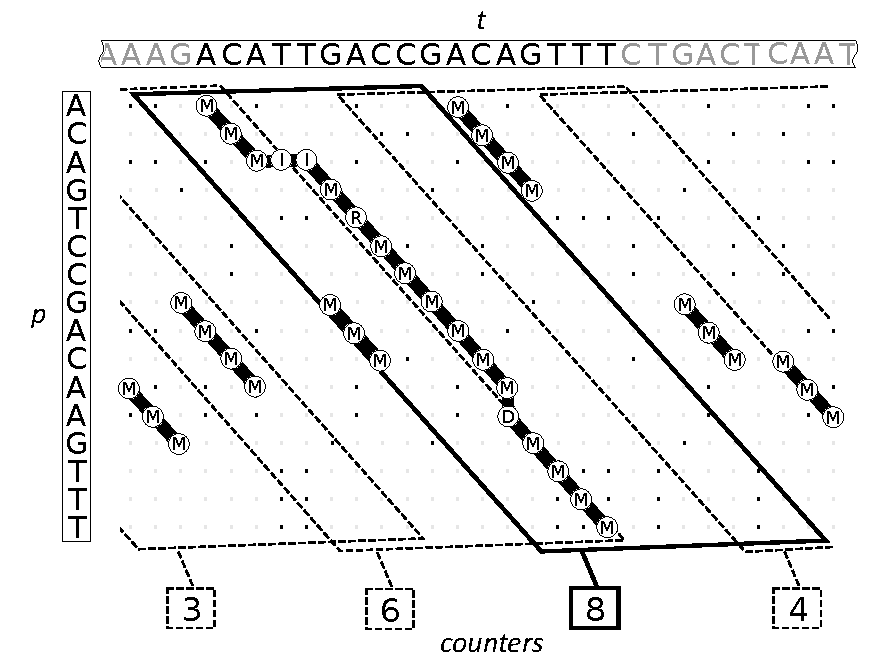
\includegraphics[scale=0.75]{figures/swift.pdf}
\end{center}
\end{figure}

This method lends itself to work in a multiple online fashion rather than offline.
The filtration stage scans the text and counts how many $q$-grams of the pattern fall into each bucket.
The verification stage then verifies only parallelograms exceeding threshold $\tau_q(m,k)$.
As long as the filter scans the text, it is necessary to remember only buckets spanning the patterns' lengths.
Conversely, the program QUASAR \citep{Burkhardt1999} uses a $q$-gram index of the text to speed up the filtration phase.
However, this implementation requires more memory, as it must keep the text index in memory and bucket the whole text.

% -----------------------------------------------------------------------------

\section{Gapped $q$-grams}
\label{sec:filtering:qgrams-gapped}

The idea of \emph{gapped $q$-grams} is to lower the correlation between consecutive $q$-grams.
The occurrence of any contiguous $q$-gram is strongly correlated to the occurrences of its preceding and following $q$-grams.
One single edit distance error affects a cluster of $q$ consecutive $q$-grams, as evidenced by the $q$-gram lemma.
Gapped $q$-grams hence define patterns of \emph{don't care positions} to skip characters at fixed positions.
Such don't care positions are immune to mismatches, but not to insertions and deletions.
Hence, this generalization of contiguous $q$-grams solves $k$-mismatches but not $k$-differences.
%Filtration specificity increases either by raising the filtering threshold or the $q$-gram length, in either cases preserving full-sensitivity.

Gapped $q$-grams rely on a generalization of the $q$-gram similarity measure (section~\ref{sec:filtering:qgrams-ext}) to \emph{subsequences}.
A subsequence is a non-contiguous sequence of symbols of a given string.
Hence, instead of substrings, filtration with gapped $q$-grams counts the number of subsequences of length $q$ common to two strings, whose positions are taken from a fixed set $Q$.
The formal definition of gapped $q$-gram follows.

\begin{definition}
A $Q$-gram is a finite sequence $Q$ of natural numbers starting with the unit element, \ie $Q \subset \N$ and $1 \in Q$.
The cardinality $|Q|$ is called the \emph{weight} of $Q$ and denoted as $w(Q)$.
The maximum element of $Q$ is named \emph{span} and indicated by $s(Q)$.
\end{definition}
%In literature, $Q$-grams are visualized as words over the alphabet $\{1,*\}$ or $\{\#,-\}$.
%I adopt the former notation and represent the $Q$-gram by the word $w \in \{1,*\}^{s(Q)}$ such that $w_j=1$ iff $j \in Q$.

\begin{figure}[h]
\begin{center}
\caption[Filtration with gapped $q$-grams]{Filtration with gapped $q$-grams.}
\label{fig:qgrams-gapped}
\begin{tikzpicture}[font=\normalsize\sffamily]

\transcript{25}{G/1/G, C/1/C, T/1/T, T/1/T, N/0/A, G/1/G, T/1/T, G/1/G, C/1/C, G/0/A, T/1/T, A/1/A, T/1/T, T/1/T, A/0/G, A/1/A, G/1/C, C/1/C, C/1/C, G/0/A, T/1/T, T/1/T, A/0/T, A/1/A, T/1/T}{5}
\band{25}
\seed{1}{25}{1}

\node[left=0.25cm of read_1] {$\Pattern$} ;
\node[left=0.25cm of genome_1] {$\Text$} ;

% Unaffected q-grams ###-#
\foreach \x in {4,9,14}
{
	\pgfmathtruncatemacro{\y}{1+Mod(\x-1,5)}
	\qgramg{\x}{$\#$, $ $, $\#$, $\#$, $\#$}{\y}{1}
}

% Covered q-grams ###-#
\foreach \x in {1,2,3,5,6,7,8,10,11,12,13,15,16,17,18,19,20,21}
{
	\pgfmathtruncatemacro{\y}{1+Mod(\x-1,5)}
	\qgramg{\x}{$\#$, $ $, $\#$, $\#$, $\#$}{\y}{0}
}

% Strikes over covered q-grams
\foreach \x in {1,2,3,5,6,7,8,10,11,12,13,15,16,17,18,20}
{
	\pgfmathtruncatemacro{\y}{5-Mod(\x-1,5)}
	\draw[strike] (qgram_\x_\y.north) -- (qgram_\x_\y.south) ;
}
\draw[strike] (qgram_21_3.north) -- (qgram_21_3.south) ;
\draw[strike] (qgram_20_4.north) -- (qgram_20_4.south) ;
\draw[strike] (qgram_19_5.north) -- (qgram_19_5.south) ;

\end{tikzpicture}
\end{center}
\end{figure}

Figure~\ref{fig:qgrams-gapped} shows an example of gapped $q$-gram.
As in the $q$-gram lemma, the threshold depends only on $Q$ and parameters $m,k$.
Indeed, the pattern of occurring $q$-grams does not depend on the text or pattern sequences but only on their transcript, \ie on the mismatch positions.
Therefore, in the following, I refer to gapped $q$-gram filtration schemes $(Q,t)$ solving $(m,k)$ instances.
As opposed to contiguous $q$-grams, don't care positions are not affected by mismatches.
Thus any gapped $q$-gram potentially yields a higher threshold than the contiguous $q$-gram of same weight.
Unfortunately, the $q$-gram lemma (\ref{lemma:qgrams}) does not give anymore a tight threshold, but only a lower bound.

Gapped $q$-grams raise hard combinatorial questions:
\begin{enumerate} %[(i)]
\item \label{enum:qgram-non-detection} Does a gapped $q$-gram yield any filtration scheme solving an $(m,k)$ instance? 
\item If the answer to question~\ref{enum:qgram-non-detection} is yes:
\begin{enumerate}
\item \label{enum:qgram-error} Which is the maximum distance $k^*$ for which full-sensitivity is guaranteed?
\item \label{enum:qgram-threshold} Which is the maximum threshold $t^*$ that guarantees full-sensitivity?
\end{enumerate}
\item \label{enum:qgram-fn} If the answer to question~\ref{enum:qgram-non-detection} is no, which is the expected sensitivity of the lossy filtration scheme?
\item \label{enum:qgram-fp} Which is the expected specificity of a filtration scheme?
%If the weight is taken as a simplified criterion predicting filtration efficiency, 
%\item \label{enum:qgram-weight} which is the maximum weight lossless shape?
\end{enumerate}

Question \ref{enum:qgram-threshold} has been first considered in \citep{Burkhardt2001,Kucherov2005},
the more general question \ref{enum:qgram-non-detection} has been introduced in \citep{Nicolas2005}, while I consider here for the first time questions \ref{enum:qgram-error}, \ref{enum:qgram-fn} and \ref{enum:qgram-fp}.
With the aim of answering these questions, I first introduce simple characteristic functions to formally define transcripts detected by gapped $q$-grams.
Afterwards, I recapitulate known results and present new exact and approximate solutions.

\subsection{Characteristic functions}

I consider any Hamming distance transcript $\sigma$ as a $m$-dimensional vector over $\Bo = \{ 0, 1 \}$.
Accordingly, I denote by $|\sigma|_0=m - \sum \sigma$ the Hamming distance of the transcript, and by $\Bo^m_k \subset \Bo^m$ the set containing all transcripts $\sigma$ \st $|\sigma|_0 = k$.
I now define the event of detection of a transcript by a filtration scheme $(Q,t)$.

\begin{definition}
\label{def:qgram-occ}
A $Q$-gram \emph{occurs} at position $i$ in a transcript $\sigma$ iff $\forall j \in Q$ $\sigma_{i+j}=1$.
\end{definition}

\begin{definition}
\label{def:qgram-detection}
A $(Q,t)$ filtration scheme \emph{detects} $\sigma$ iff the $Q$-gram occurs at least $t$ times in $\sigma$.
\end{definition}

\subsubsection{Boolean functions}

I introduce boolean functions to characterize the set of transcripts detected by filtration schemes of the form $(Q,0)$ according to definition \ref{def:qgram-detection}.
The utility of these functions is manyfold.
In section \ref{sub:qgram-optimal-threshold}, I use them directly within an ILP that computes an exact solution to \textsc{Optimal Threshold} and thus answers \textsc{Non Detection}.
In section \ref{sub:qgram-specificity}, I reduce the estimation of filtration sensitivity to a counting problem on boolean functions.

Let $T_{Q}^{m}: \Bo^m \rightarrow \Bo$ denote a \emph{boolean function} such that $T_{Q}^{m}(\sigma)$ is true iff the $Q$-gram occurs at least one time in a transcript $\sigma$ of length $m$.
I define such boolean function as the disjunction
\begin{equation}
\label{eq:qgram-bool}
T_{Q}^{m}(\sigma) = \bigvee_{i=1}^{m-s(Q)+1} \bigwedge_{j \in Q} \sigma_{i+j}
\end{equation}
where each \emph{clause} of $T_{Q}^{m}$ represents a single possible occurrence of $Q$ in $\sigma$.
According to definition \ref{def:qgram-occ}, filtration scheme $(Q,t)$ detects $\sigma$ iff $\sigma$ satisfies at least $t$ clauses of $T_{Q}^{m}$.
%The seed boolean function $T_{Q}^{m}$ describes the computation performed by the seed automaton $A_Q$ on all transcripts of length $m$.
I define an analogous boolean function for a $Q$-gram family $F$ as the disjunction
\begin{equation}
\label{eq:family-bool}
T_{F}^{m}(\sigma) = \bigvee_{Q_i \in F} T_{Q_i}^{m}(\sigma)
\end{equation}
By definition, $T_{Q}^{m}$ and $T_{F}^{m}$ are \emph{monotone nondecreasing} boolean functions in \emph{disjunctive normal form} (\emph{DNF}).
Since all monotone boolean functions in DNF are minimal, $T_{Q}^{m}$ and $T_{F}^{m}$ are \emph{minimal}.

\subsubsection{Pseudo-boolean functions}

I now consider pseudo-boolean functions, corresponding to functions \ref{eq:qgram-bool} and \ref{eq:family-bool}, to associate a filtration threshold to each transcript.
The following pseudo-boolean functions exhibit the combinatorial properties of super or submodularity, which are important in respect to their optimization.

Let the function $t_{Q}^{m}: \Bo^m \rightarrow \N_0$ be the boolean function $T_{Q}^{m}$ acting on $\N_0$.
I define such \emph{pseudo-boolean function} as
\begin{equation}
\label{eq:qgram-pseudo}
t_{Q}^{m}(\sigma) = \sum_{i=1}^{m-s(Q)+1} \prod_{j \in Q}\sigma_{i+j}
\end{equation}
Here $t_{Q}^{m}(\sigma)$ \emph{counts} how many times a $Q$-gram occurs in a transcript $\sigma$ of length $m$.
It is useful to define the complementary function $\bar{t}_{Q}^{m}$, counting how many times a $Q$-gram does not occur in a transcript $\sigma$, as
\begin{equation}
\label{eq:qgram-pseudoneg}
\bar{t}_{Q}^{m}(\sigma) = m - s(Q) + 1 - t_{Q}^{m}(\sigma)
\end{equation}
Analogously, I define a pseudo-boolean function for a $Q$-gram family $F$
\begin{equation}
\label{eq:family-pseudo}
t_{F}^{m}(\sigma) = \sum_{Q_i \in F} t_{Q_i}^{m}(\sigma)
\end{equation}
along with its complementary function
\begin{equation}
\label{eq:family-pseudoneg}
\bar{t}_{F}^{m}(\sigma) = \sum_{Q_i \in F}{(m - s(Q_i) + 1)} - t_{F}^{m}(\sigma)
\end{equation}

All of the above functions expose important properties which lead to approximate solutions.
\emph{Nondecreasing monotonicity} of functions $t_{Q}^{m}$ and $t_{F}^{m}$ follow from nondecreasing monotonicity of their boolean counterparts $T_{Q}^{m}$ and $T_{F}^{m}$. Consequently $\bar{t}_{Q}^{m}$ and $\bar{t}_{F}^{m}$ are \emph{monotone nonincreasing}.
From definition~\ref{eq:supermodularity}, function $t_{Q}^{m}$ is \emph{supermodular}, thus it follows that $\bar{t}_{Q}^{m}$ is \emph{submodular}.
Since super and submodular functions are closed under non-negative linear combination, functions $t_{F}^{m}$ and $\bar{t}_{F}^{m}$ are respectively super and submodular.

\subsection{Full-sensitivity}
\label{sub:qgram-full-sensitivity}

%\textsc{Non Detection}~\citep{Nicolas2005} asks the question: does a given $Q$-gram solve a $(m,k)$ instance?

\subsubsection{Problem definition}

\paragraph{}
\begin{tabular}{rl}
{\bf Instance}	&	A $Q$-gram, a $(m,k)$ instance. \\
{\bf Question}	&	Does it exist a transcript $\sigma \in \Bo^{m}_{k}$ such that $T_{Q}^{m}(\sigma)$ is false? \\
\end{tabular}
\\

\subsubsection{Hardness results}

\cite{Nicolas2005} show that \textsc{Non Detection} is \emph{strongly} NP-complete by giving an indirect reduction of \textsc{Exact Cover by 3-Sets} to \textsc{Non Detection}.
Strong NP-completeness implies that no \emph{FPTAS} nor any \emph{pseudo-polynomial} algorithm for \textsc{Non Detection} exist, under the assumption that $P \neq NP$.
This fact motivates me to give ILP or approximate solutions to optimization and counting problems related to \textsc{Non Detection}.

\subsection{Minimum lossy distance}
\label{sub:qgram-min-lossy-distance}

\subsubsection{Problem definition}

\paragraph{}
\begin{tabular}{rl}
{\bf Instance}	&	A $Q$-gram, an integer $m > 0$.\\
{\bf Solution}	&	The smallest integer $k^*$ such that \textsc{Non Detection} for $Q$, $(m,k^*)$ answers \emph{no}.\\
\end{tabular}
\\

Recalling pseudo-boolean function \ref{eq:qgram-pseudo}, I define this problem as the minimization of a linear function subject to submodular constraints
\begin{equation}
\begin{array}{ll}
\min & |\sigma|_0			\\
w.r.t.								\\
& \sigma \in \Bo^m					\\
& \bar{t}_{Q}^{m}(\sigma) = 0	\\
\end{array}
\end{equation}

\subsubsection{ILP solution}

I reduce the problem to \textsc{Minimum Set Cover} \citep{Vazirani2001} and solve it with the following ILP
\begin{equation}
\begin{array}{ll}
\min & \sum \bar{\sigma}	\\
w.r.t.						\\
& \sigma \in \Bo^m			\\
& A\sigma \geq b	\\
\end{array}
\end{equation}
where the value $A_{ij}$ of the coefficient matrix $A$ is defined as
\begin{equation}
A_{ij} = 
\left\{
	\begin{array}{ll}
		1  & \mbox{if } i-j+1 \in Q		\\
		0  & \mbox{if } i-j+1 \notin Q	\\
	\end{array}
\right.
\end{equation}
and $b$ is the unitary vector $\mathbb{1}^{m - s(Q) + 1}$.
Given the ILP solution $\bar{\sigma}^*$, the minimum distance for which the $Q$-gram is lossy is $k^* = |\sigma^*|_0$.

\begin{observation}
Contiguous $q$-grams provide an interesting special case of this ILP.
If $A$ has the \emph{Consecutive Ones Property}, it is \emph{totally unimodular} \citep{Fulkerson1964}.
The \emph{polytope} defined by a totally unimodular coefficient matrix is \emph{integral}.
Hence the optimal solution of the relaxed LP is also the optimal solution of the original ILP.
\end{observation}

\subsubsection{APX solution}

I adapt the greedy algorithm by \citeauthor{Chvatal1979} to compute an approximate solution to \textsc{Minimum Set Cover}.
Algorithm \ref{alg:qgram-maxdist-apx} computes via \emph{gradient descent} a solution with an APX-ratio of $H_{w(Q)}$ \citep{Chvatal1979}.

\begin{figure*}[h]
\begin{center}
\begin{minipage}[t]{.8\textwidth}
\begin{algorithm}[H]
\Algorithm{MinLossyDistance}{$Q,m$}
\begin{tabular}{ll}
\textbf{Input}  & $Q$ : $Q$-gram sequence\\
				& $m$ : integer denoting the pattern length\\
\textbf{Output} & integer indicating the minimum lossy distance\\
\end{tabular}
\begin{algorithmic}[1]
\State {$k \gets 0$}
\State {$\sigma \gets \mathbb{1}^m$}
\While {$t^m_Q(\sigma) > 0$}
	\State {i \gets $ \argmax_{j=1}^{m} \frac{\partial t^m_Q(\sigma)}{\partial \sigma_j}$}
	\State {$\sigma_i \gets 0$}
	\State {$k \gets k + 1$}
\EndWhile
\State \Return $k$
\end{algorithmic}
\label{alg:qgram-maxdist-apx}
\end{algorithm}
\end{minipage}
\end{center}
\end{figure*}

\subsection{Optimal threshold}
\label{sub:qgram-optimal-threshold}

%Which is the highest $Q$-gram threshold $t^*$ that guarantees full-sensitivity for a $()$?
%This problem has been introduced in \citep{Burkhardt2001}. %and generalized in \citep{Kucherov2005}.

\subsubsection{Problem definition}

\paragraph{}
\begin{tabular}{rl}
{\bf Instance}	&	A $Q$-gram, a $(m,k)$ instance.\\
{\bf Solution}	&	The largest integer $t^*$ such that $(Q,t^*)$ solves $(m,k)$.\\
\end{tabular}
\\

Recalling $Q$-gram pseudo-boolean functions \ref{eq:qgram-pseudo}, I define \textsc{Optimal Threshold} as the minimization of a supermodular function subject to linear constraints
\begin{equation}
\begin{array}{ll}
\min & t_{Q}^{m} (\sigma)			\\
w.r.t.								\\
& \sigma \in \Bo^m_k				\\
\end{array}
\end{equation}

Recalling $Q$-gram pseudo-boolean functions \ref{eq:qgram-pseudoneg}, I consider the \emph{complementary} \textsc{Optimal Threshold} problem as the maximization of a submodular function subject to linear constraints:
\begin{equation}
\begin{array}{ll}
\max & \bar{t}_{Q}^{m} (\sigma)		\\
w.r.t.								\\
& \sigma \in \bar{\Bo}^m_k			\\
\end{array}
\end{equation}

\subsubsection{Previous results}

\textsc{Optimal Threshold} is fixed-parameter tractable (FPT) in the span of the $Q$-gram.
 \cite{Burkhardt2001} give a DP algorithm computing the optimal threshold in time $\Oh(m \cdot k \cdot 2^{s(Q)})$.
\cite{Kucherov2005} give an extension for $Q$-gram families.

\subsubsection{Exact ILP solution}

I reduce this problem to \textsc{maximum coverage} \citep{Vazirani2001} and solve it with the following ILP
\begin{equation}
\begin{array}{ll}
\max & \sum c_j					\\
w.r.t.							\\
& \sigma \in \Bo^m_k			\\
& c \in \Bo^{m - s(Q) + 1}		\\
& \sigma_i \geq c_j				\\
\end{array}
\end{equation}
where variable $c_j$ indicates the truthfulness of the $j$-th clause in $T_{Q}^{m}$.
From the ILP solution $c^*$, I derive the exact solution to \textsc{Optimal Threshold} as $t^* = m - s(Q) + 1 - \sum c^*$.

\subsubsection{APX solution}

Algorithm~\ref{alg:qgram-threshold-apx} computes via \emph{gradient descent} an approximate solution to \textsc{Optimal Threshold}.
This algorithm has an APX-ratio of $1 + 1/e$ \citep{Vazirani2001} for the complementary \textsc{Optimal Threshold} problem.
The same \emph{absolute error} applies to \textsc{Optimal Threshold}.

\begin{figure*}[h]
\begin{center}
\begin{minipage}[t]{.8\textwidth}
\begin{algorithm}[H]
\Algorithm{OptimalThreshold}{$Q,m,k$}
\begin{tabular}{ll}
\textbf{Input}  & $Q$ : $Q$-gram sequence\\
				& $m$ : integer denoting the pattern length\\
				& $k$ : integer denoting the mismatches threshold\\
\textbf{Output} & integer indicating the maximum lossless threshold\\
\end{tabular}
\begin{algorithmic}[1]
\State {$\sigma \gets \mathbb{1}^m$}
\While {$k > 0$}
	\State {i \gets $ \argmax_{j=1}^{m} \frac{\partial \bar{t}^m_Q(\sigma)}{\partial \sigma_j}$}
	\State {$\sigma_i \gets 0$}
	\State {$k \gets k - 1$}
\EndWhile
\State \Return $m - s(Q) + 1 - \bar{t}^m_Q(\sigma)$
\end{algorithmic}
\label{alg:qgram-threshold-apx}
\end{algorithm}
\end{minipage}
\end{center}
\end{figure*}

\subsection{Specificity}
\label{sub:qgram-specificity}

Which is the expected specificity of a filtration scheme $(Q,t)$?
Assuming the text to be generated according to the uniform Bernoulli model, the expected specificity of a filtration scheme is proportional to the number of detected transcripts.
Among full-sensitive filtration schemes, one that maximizes the expected specificity is preferable.

\subsubsection{Problem definition}

\paragraph{}
\begin{tabular}{rl}
{\bf Instance}	&	A filtration scheme $(Q,t)$, a $(m,k)$ instance.\\
%{\bf Solution}	&	The number of transcripts $\sigma \in \bar{\Bo}^{m}_{k}$ \st $t_{Q}^{m}(\sigma) \geq t$\\
{\bf Solution}	&	The number of transcripts $\sigma \in \Bo^{m}$ \st $t_{Q}^{m}(\sigma) \geq t$\\
\end{tabular}
\\

%False positives are true points of the boolean function \ref{eq:qgram-bool} which have weight inferior to $m-k$ and satisfy more than $t$ clauses of $T_{Q}^{m}$.
%Hence, I define the function $\text{FP}_{k}^{m}$ counting the number of false positives of filter $(Q,t)$ in instance $(m,k)$ as
%\begin{equation}
%\text{FP}_{k}^{m}(Q,t) = \sum_{\sigma \in {\bar{\Bo}^{m}_{k}}} t_{Q}^{m}(\sigma) \geq t
%\end{equation}

\subsubsection{FPRAS solution}

I am interested in the number of transcripts:
\begin{equation}
\text{\#P}^{m}(Q,t) = | \{ \sigma \in \Bo^{m} : t_{Q}^{m}(\sigma) \geq t \} |
\end{equation}
For threshold $t=1$, this number is simply the number of true assignments of $T_{Q}^{m}$:
\begin{equation}
\text{\#P}^{m}(Q,1) = | \{ \sigma \in \Bo^{m} : T_{Q}^{m}(\sigma) \} |
\end{equation}
\citeauthor{Karp1989} introduce a \emph{fully polynomial-time randomized approximation scheme} (FPRAS) \citep{Vazirani2001} to count the number of true assignments of a boolean function in DNF \citep{Karp1989}.
This method is known as \emph{importance sampling} \citep{Vazirani2001}.
Algorithm~\ref{alg:qgram-specificity} works for an arbitrary threshold.

\begin{figure*}[h]
\begin{center}
\begin{minipage}[t]{.8\textwidth}
\begin{algorithm}[H]
\Algorithm{TranscriptsDetected}{$Q,t,m$}
\begin{tabular}{ll}
\textbf{Input}  & $Q$ : $Q$-gram sequence\\
				& $t$ : integer denoting the threshold\\
				& $m$ : integer denoting the pattern length\\
\textbf{Output} & integer indicating the number of transcripts detected\\
\end{tabular}
%\begin{algorithmic}[1]
%\State {\Return 0}
%\end{algorithmic}
\label{alg:qgram-specificity}
\end{algorithm}
\end{minipage}
\end{center}
\end{figure*}

%\subsection{Sensitivity and specificity}
%and \ref{enum:qgram-fn}.

%\subsection{Optimal gapped $q$-grams}
%
%Introduced in \citep{Nicolas2005}.
%
%\subsubsection{Problem definition}
%
%\paragraph{}
%\begin{tabular}{rl}
%{\bf Instance}	&	A finite set $S$ of transcripts.\\
%{\bf Solution}	&	A $Q$-gram that detects all transcripts of $S$.\\
%{\bf Measure}	&	The weight $w(Q)$ of the $Q$-gram.\\
%\end{tabular}
%\\
%
%Given a set of transcripts, find the $Q$-gram of maximum weight detecting all transcripts.
%This applies to the DNA Homology Search Framework as well.
%%The MWLS is not the optimal seed for approximate string matching filtration nor for sequence homology filtration.
%%On the one hand the weight is just an estimator of sensibility regardless of threshold, on the other hand filtration speed decreases with increasing weight.
%
%\subsubsection{Hardness and inapproximability results}
%
%Nicolas et al. \citep{Nicolas2005} perform an approximation preserving reduction from \textsc{Maximum Independent Set}.
%MWLS is NP-hard and APX-hard within $(|S|)^{0.25 - \epsilon}$ unless $P = NP$.
%If $S = \Bo^{m}_{k}$, $|S| = \binom{m}{k}$.
%
%\subsubsection{Branch-and-bound search}
%
%Burkhardt et al. \citep{Burkhardt2001} bounding criterion. If $Q_1 \subseteq Q_2$, then $t_{Q_2}(m,k) \leq t_{Q_1}(m,k)$.
%Such bounding criterion allows to discard parts of the search space which do not solve the considered $(m,k)$ instance.
%%The search space of seed families is more dense than the search space of single seeds (i.e. almost all seed families solve a give Non Detection instance). Thus search space pruning would not be as effective.

% -----------------------------------------------------------------------------

%\section{Verification methods}
%\label{sec:verification}
%\section{Myers' bit-vector algorithm}
%\subsection{Banded Myers' bit-vector algorithm}
%\subsection{Increased bit-parallelism using SIMD instructions}

% -----------------------------------------------------------------------------

\section{Evaluation}
\label{sec:filtering:evaluation}

In this section, I show the results of an experimental evaluation of all filtration methods exposed so far.
I consider seed filtration schemes with exact, 1 and 2-approximate seeds (Exact, 1-Apx and 2-Apx seeds), contiguous $q$-grams filtration schemes using the maximum lossless value of $q$ for a threshold of 1 ($q$-Grams, $t \geq 1$) and 4 ($q$-Grams, $t \geq 4$).
For indexed filters, I use the $q$-gram index with $q=10$ (see \ref{sec:index:qgram}).
To perform edit distance verifications, I use a banded version of the Myers' algorithm \citep{Myers1999}.
As text, I take the \emph{C.~elegans} reference genome (WormBase WS195), \ie a collection of 6 DNA strings of about 100~Mbp total length.
As patterns, I extrapolated $200k$ DNA sequences of length 100~bp from an Illumina sequencing run (Sequence Read Archive ID SRR065390).

All experiments run on a desktop computer running Linux~3.10.11, equipped with one Intel\textsuperscript{\textregistered} Core i7-4770K CPU @ 3.50\,GHz, 32\,GB RAM and a 2\,TB HDD @ 7200\,RPM.
I repeated the experiment for $k$-mismatches and $k$-differences, varying $k$ in the range $[1,10]$.
I measured the runtime of the filtration phase only, and then of the filtration plus verification phase.
The plots show always \emph{average} runtimes (or values) per pattern.

\subsection{Runtime}

Figure \ref{fig:filter-runtime-hamming-celegans} shows the results for $k$-mismatches.
Exact seeds are the best filtration method for $k \leq 7$, mainly due to their superior filtration speed, while 1-approximate seeds are better for $k \geq 8$.
2-Approximate seeds start to dominate exact seeds only for $k \geq 10$, \ie they provide too strong filtration on this text.
Both $q$-gram filtration schemes are always slower than 1-approximate seeds.
It can be seen that enforcing $t \geq 4$ improves the total runtime for those instances where $t \geq 1$ renders the filter too weak.

Figure \ref{fig:filter-runtime-edit-celegans} shows the results for $k$-differences.
The more involved edit distance verification slightly fills the gap between exact seeds and contiguous $q$-grams, yet exact seeds continue to be always the fastest alternative.

\begin{figure}[h]
\begin{center}
\caption[Filters runtime on $k$-mismatches]{Filters runtime on $k$-mismatches. Pattern length is fixed to 100. Dashed lines represent filtration time only.}
\label{fig:filter-runtime-hamming-celegans}
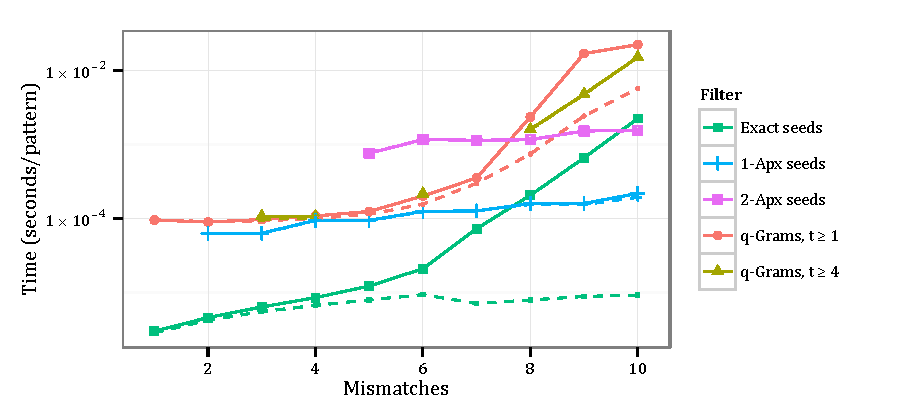
\includegraphics{filter_runtime.dna.celegans.hamming.100}
\end{center}
\end{figure}

\begin{figure}[h]
\begin{center}
\caption[Filters runtime on $k$-differences]{Filters runtime on $k$-differences. Pattern lengths are fixed to 100~bp. Dashed lines represent filtration time only.}
\label{fig:filter-runtime-edit-celegans}
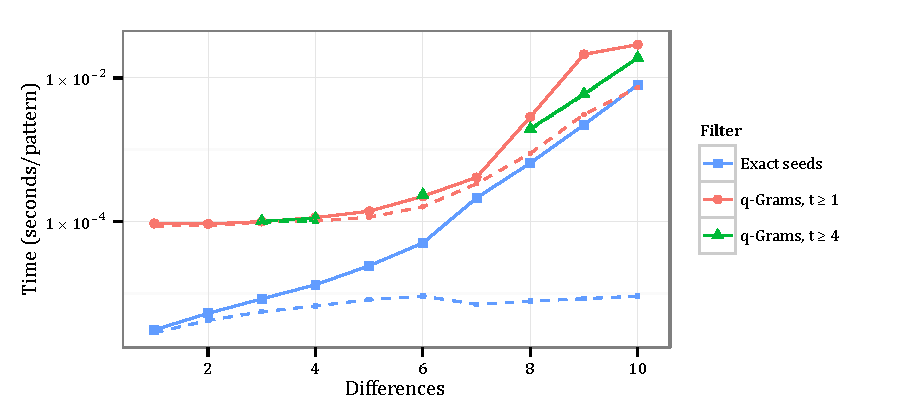
\includegraphics{filter_runtime.dna.celegans.edit.100}
\end{center}
\end{figure}

\subsection{Verification versus filtration}

Figure \ref{fig:filter-ratio-hamming-celegans} shows the ratios between the runtimes of the verification and filtration phases of each filtration scheme.
For $k \leq 6$, all schemes spend more time on filtration rather than verification.
The weakest scheme, filtration with exact seeds, shows the closest ratio to 1.
As shown in the runtime plots (figures \ref{fig:filter-runtime-hamming-celegans}-\ref{fig:filter-runtime-edit-celegans}), quick filtration pays off for low error rates.
Here, a quicker full-text index would be beneficial.
For $k \geq 7$, contiguous $q$-grams with $t \geq 1$ show the closest ratio to 1, nonetheless the fastest alternative is provided by filtration with 1-approximate seeds, for which only 10\,\% of the runtime goes in verifications.
Here, a judicious mix of exact and 1-approximate seeds could improve the total runtime.
The ratios for $k$-difference show analogous patterns (data not shown).

\begin{figure}[h]
\begin{center}
\caption[Ratio on $k$-mismatches]{Ratio on $k$-mismatches. Pattern lengths are fixed to 100~bp.}
\label{fig:filter-ratio-hamming-celegans}
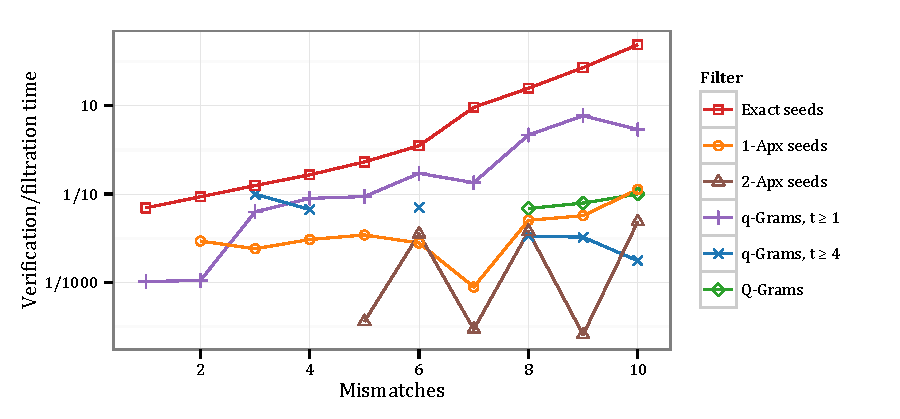
\includegraphics{filter_ratio.dna.celegans.hamming.100}
\end{center}
\end{figure}

%\begin{figure}[h]
%\begin{center}
%\caption[Ratio on $k$-differences]{Ratio on $k$-differences. Pattern length is fixed to 100.}
%\label{fig:filter-ratio-edit-celegans}
%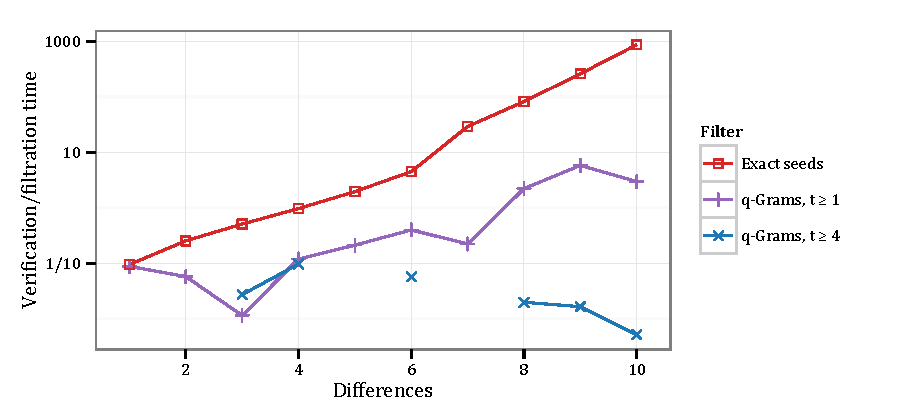
\includegraphics{filter_ratio.dna.celegans.edit.100}
%\end{center}
%\end{figure}

\subsection{Positive predictive value}

Instead of measuring filtration specificity, as introduced in section \ref{intro:filtering:spec-sens}, I measure the \emph{positive predictive value} (PPV).
As shown in table \ref{tab:filter:ppv}, I define \emph{true positives} (TP), \emph{false positives} (FP), \emph{true negatives} (TN), or \emph{false negatives} (FN) in terms of the number of verifications $V$ triggered by the filtration phase and the number of approximate occurrences $C$ passing the verification phase.
For a more precise experimental evaluation, $C$ counts as distinct occurrences one single approximate occurrence reported multiple times.
Therefore, I define the PPV as:
\begin{eqnarray}
\frac{|TP_f(t)|}{|TP_f(t)| + |FP_f(t)|} = \frac{C}{V}
\end{eqnarray}

\begin{table}[t]
\begin{center}
\caption[Measurement of filtering methods efficiency]{Measurement of filtering methods efficiency. $V$ counts the number of verifications, $C$ the number of approximate occurrences, and $||T||$ the total length of the text collection. Since all considered filtering methods are full-sensitive, the number of false negatives is always 0.}
\begin{tabular}{rcc}
\toprule
  & Positive & Negative\\
\midrule
True & $C$ & $||T|| - C$ \\
False & $V - C$ & 0		\\
\bottomrule
\end{tabular}
\label{tab:filter:ppv}
\end{center}
\end{table}

Figure \ref{fig:filter-ppv-hamming-celegans} shows the results for $k$-mismatches.
As expected, 2-approximate seeds have always the highest PPV, followed by 1-approximate seeds.
The PPV of contiguous $q$-grams with $t \geq 1$ oscillates around that one of exact seeds.
In particular, when $t$ approaches $1$, \eg for $k = 9$, the PPV of contiguous $q$-grams stays below that one of exact seeds.
Enforcing $t \geq 4$ boosts the PPV of contiguous $q$-grams to that one of 1-approximate seeds.
The PPVs for $k$-difference show analogous patterns (data not shown).

\begin{figure}[h]
\begin{center}
\caption[Filters specificity on $k$-mismatches]{Filters specificity on $k$-mismatches. Pattern lengths are fixed to 100~bp.}
\label{fig:filter-ppv-hamming-celegans}
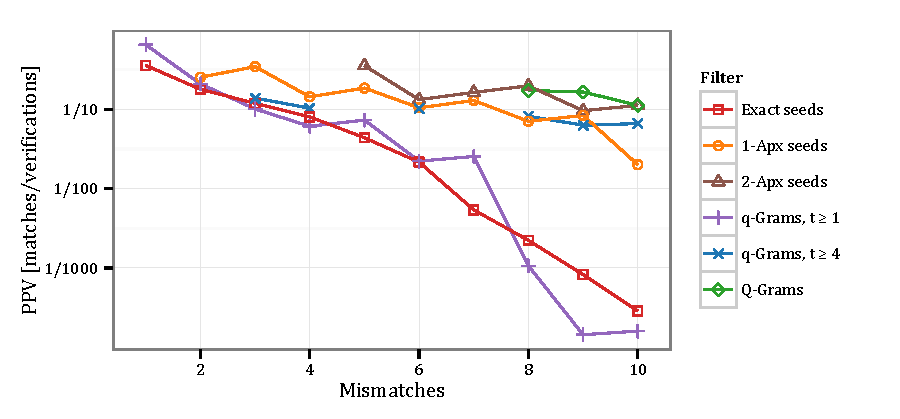
\includegraphics{filter_ppv.dna.celegans.hamming.100}
\end{center}
\end{figure}

%\begin{figure}[h]
%\begin{center}
%\caption[Filters specificity on $k$-differences]{Filters specificity on $k$-differences. Pattern length is fixed to 100.}
%\label{fig:filter-ppv-edit-celegans}
%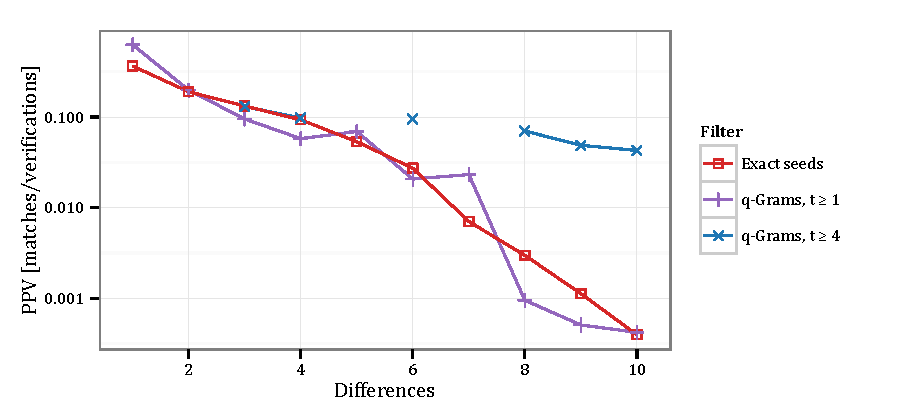
\includegraphics{filter_ppv.dna.celegans.edit.100}
%\end{center}
%\end{figure}
